\documentclass[12pt,]{article}
\usepackage{lmodern}
\usepackage{amssymb,amsmath}
\usepackage{ifxetex,ifluatex}
\usepackage{fixltx2e} % provides \textsubscript
\ifnum 0\ifxetex 1\fi\ifluatex 1\fi=0 % if pdftex
  \usepackage[T1]{fontenc}
  \usepackage[utf8]{inputenc}
\else % if luatex or xelatex
  \ifxetex
    \usepackage{mathspec}
    \usepackage{xltxtra,xunicode}
  \else
    \usepackage{fontspec}
  \fi
  \defaultfontfeatures{Mapping=tex-text,Scale=MatchLowercase}
  \newcommand{\euro}{€}
\fi
% use upquote if available, for straight quotes in verbatim environments
\IfFileExists{upquote.sty}{\usepackage{upquote}}{}
% use microtype if available
\IfFileExists{microtype.sty}{%
\usepackage{microtype}
\UseMicrotypeSet[protrusion]{basicmath} % disable protrusion for tt fonts
}{}
\usepackage[margin=1in]{geometry}
\usepackage{longtable,booktabs}
\ifxetex
  \usepackage[setpagesize=false, % page size defined by xetex
              unicode=false, % unicode breaks when used with xetex
              xetex]{hyperref}
\else
  \usepackage[unicode=true]{hyperref}
\fi
\hypersetup{breaklinks=true,
            bookmarks=true,
            pdfauthor={},
            pdftitle={},
            colorlinks=true,
            citecolor=blue,
            urlcolor=black,
            linkcolor=black,
            pdfborder={0 0 0}}
\urlstyle{same}  % don't use monospace font for urls
\setlength{\parindent}{0pt}
\setlength{\parskip}{6pt plus 2pt minus 1pt}
\setlength{\emergencystretch}{3em}  % prevent overfull lines
\setcounter{secnumdepth}{0}

%%% Use protect on footnotes to avoid problems with footnotes in titles
\let\rmarkdownfootnote\footnote%
\def\footnote{\protect\rmarkdownfootnote}

%%% Change title format to be more compact
\usepackage{titling}

% Create subtitle command for use in maketitle
\newcommand{\subtitle}[1]{
  \posttitle{
    \begin{center}\large#1\end{center}
    }
}

\setlength{\droptitle}{-2em}
  \title{}
  \pretitle{\vspace{\droptitle}}
  \posttitle{}
  \author{}
  \preauthor{}\postauthor{}
  \date{}
  \predate{}\postdate{}

\usepackage{setspace}
\usepackage{todonotes}
\usepackage{color}
\usepackage{rotating}
\usepackage{fancyhdr}
\pagestyle{fancy}
\chead{\color{red}THIS MANUSCRIPT HAS NOT UNDERGONE PEER REVIEW}
\lhead{}
\rhead{}


\begin{document}

\maketitle

\thispagestyle{fancy}
\begin{singlespace}

\begin{center}
\large{\textbf{Environmental responses, not species interactions, determine species synchrony in natural plant communities}}

\renewcommand*{\thefootnote}{\fnsymbol{footnote}}

\vspace{1em}

\normalsize{Andrew T. Tredennick\textsuperscript{1}\footnote{Correspondence: Email: atredenn@gmail.com}, Claire de Mazancourt\textsuperscript{2}, Michel Loreau\textsuperscript{2}, and Peter B. Adler\textsuperscript{1}}

\vspace{1em}

\textit{\small{\textsuperscript{1}Department of Wildland Resources and the Ecology Center, 5230 Old Main Hill, Utah State University, Logan, Utah 84322 USA}}

\textit{\small{\textsuperscript{2}Centre for Biodiversity Theory and Modelling, Theoretical and Experimental Ecology Station, CNRS and Paul Sabatier University, Moulis, 09200, France}}

\end{center}

\end{singlespace}\renewcommand*{\thefootnote}{\arabic{footnote}}

\setcounter{footnote}{0}

\begin{abstract}
Temporal asynchrony among species is an important mechanism through which diversity can stabilize ecosystem functioning, but identifying the mechanisms that determine synchrony remains a challenge.
Here, we refine and test theory showing that synchrony depends on three factors: species responses to environmental variation, interspecific competition, and demographic stochasticity. We then conduct simulation experiments with empirical population models to quantify the relative importance of these factors in five plant communities.
Simulation experiments showed that the average synchrony of per capita growth rates, which can range from 0 (perfect asynchrony) to 1 (perfect synchrony), was higher when environmental variation was present (0.62) rather than absent (0.43).
Removing interspecific competition and demographic stochasticity had small effects on synchrony. In these plant communities, where species interactions and demographic stochasticity have little influence, synchrony reflects the covariance in species responses to the environment.

\vspace{2em}

\noindent{}\textbf{Keywords}\\
\noindent{}synchrony, compensatory dynamics, environmental stochasticity, demographic stochasticity, interspecific competition, stability
\end{abstract}

\setlength{\parindent}{5ex}

\subsection{INTRODUCTION}\label{introduction}

Ecosystems are being transformed by species extinctions (Cardinale et
al. 2012), changes in community composition (Vellend et al. 2013,
Dornelas et al. 2014), and anthropogenic environmental change (Vitousek
et al. 1997), impacting the provisioning and stability of ecosystem
services (Loreau et al. 2001, Hooper et al. 2005, Rockstrom et al.
2009). Experiments have provided compelling evidence that decreases in
species richness will decrease productivity (Tilman et al. 2001) and the
temporal stability of productivity (Tilman et al. 2006, Hector et al.
2010). The stabilizing effect of species richness stems from individual
species responding to environmental fluctuations (environmental
stochasticity), or fluctuating asynchronously because of random chance
events (demographic stochasticity) (Isbell et al. 2009, Hector et al.
2010, {{de Mazancourt}} et al. 2013). Species richness affects synchrony
because larger species pools are more likely to contain species that
respond disimilarly to environmental conditions (Yachi and Loreau 1999),
implying that species losses will reduce ecosystem stability. Even
without species losses, abiotic homogenization can weaken compensatory
dynamics and, in turn, decrease temporal stability of ecosystem
functioning (Hautier et al. 2014). Predicting the impacts of global
change requires a mechanistic understanding of species synchrony in
natural settings.

Theory identifies the three main determinants of species synchrony as
environmental stochasticity, demographic stochasticity, and
interspecific competition (Loreau and {{de Mazancourt}} 2008, 2013,
Gonzalez and Loreau 2009). For example, in a community composed of large
(no demographic stochasticity) and weakly interacting (no interspecific
competition) populations, community-wide species synchrony should be
determined by the covariance of species' responses to the environment
(Loreau and {{de Mazancourt}} 2008). However, such a prediction relies
on a relatively simple population model and only holds under two
assumptions: (i) species' responses to the environment are similar in
magnitude and (ii) all species have similar growth rates. Whether such
theoretical predictions hold in natural communities where species
differences are unlikely to be symmetrical remains unkown: no study has
explicitly tested theory on the drivers of species synchrony in natural
communities.

In grasslands, most empirical studies have focused on whether species
synchrony is primarily an outcome of species-specific responses to
environmental conditions (Hautier et al. 2014) or competition (Gross et
al. 2014). Even beyond grassland studies, whether competition or
environmental responses drive compensatory dynamics remains
controversial (reviewed in Gonzalez and Loreau 2009). In part,
controversy remains because quantifying the relative strengths of each
driver on the degree of synchrony from community time series (e.g.,
Houlahan et al. 2007) is impossible. This is because an unbiased null
expectation for synchrony does not exist (Loreau and {{de Mazancourt}}
2008) and observed synchrony can arise from non-unique combinations of
factors (Ranta et al. 2008). For example, weak synchrony of population
abundances could reflect positive environmental correlations
(synchronizing effect) offset by strong competition (desynchronizing
effect), or negative environmental correlations and weak competition.

The best way to quantify the effects of environmental stochasticity,
demographic stochasticity, and interspecific competition is to remove
them one-by-one, and in combination. In principle, this could be done in
an extremely controlled laboratory setting, but empirically-based models
of interacting populations, fit with data sets from natural communities,
offer a practical alternative. For example, Mutshinda et al. (2009) fit
a dynamic population model to several community time series of insect
and bird abundances. They used a statistical technique to decompose
temporal variation into competition and environmental components, and
found that postively correlated environmental responses among species
determined community dynamics. While a major step forward, Mutshinda et
al.'s (2009) modeling technique relied on abundance data that may or may
not reliably capture competitive interactions that occur at the
individual level. Furthermore, although Mutshinda et al. (2009)
quantified the relative importance of environmental stochasticity and
competition to explain the observed variation of species synchrony, they
did not use the model to quantify how much synchrony would change when
each factor is removed.

Here, we use multi-species population models fit to long-term
demographic data from five semi-arid plant communities to test theory on
the drivers of species synchrony. Our objectives are to (1) derive and
test theoretical predictions of species synchrony and (2) determine the
relative influence of environmental stochasticity, demographic
stochasticity, and interspecific competition on species synchrony in
natural plant communities. To achieve these objectives, we first refine
theory that has been used to predict the effects of species richness on
ecosystem stability ({{de Mazancourt}} et al. 2013) and species
synchrony (Loreau and {{de Mazancourt}} 2008) to generate predictions of
community-wide species synchrony under two limiting cases derived from
the dynamics of individual species in monoculture. We then confront our
theoretical predictions with simulations from the empirically-based
population models. Second, we use the multi-species population models to
perform simulation experiments that isolate the effects of environmental
stochasticity, demographic stochasticity, and interspecific competition
on community-wide species synchrony. Given that our population models
capture the essential features of community dynamics important to
synchrony (density-dependence, and demographic and environmental
stochasticity), and that these models successfully reproduce observed
community dynamics (Chu and Adler 2015), perturbing the models can
reveal the processes that determine species synchrony in our focal
grassland communities.

\subsection{THEORETICAL MODEL}\label{theoretical-model}

\subsubsection{The model}\label{the-model}

While existing theory has identified the factors driving synchrony, we
do not have a simple expression to predict synchrony in a particular
community with all factors operating simultaneously. However, we can
derive analytical predictions for species synchrony under special
limiting cases. We focus on synchrony of per capita growth rates, rather
than abundances, because growth rates represent the instantaneous
response of species to the environment and competition, and are less
susceptible to the legacy effects of drift and disturbance (Loreau and
{{de Mazancourt}} 2008). We present equivalent results for synchrony of
species abundances in the Online Supporting Information, and show that
they lead to the same overall conclusions as synchrony of per capita
growth rates. Following Loreau and {{de Mazancourt}} (2008) and {{de
Mazancourt}} et al. (2013), we define population growth, ignoring
observation error, as

\begin{align}
r_i(t) &= \text{ln}N_i(t+1) - \text{ln}N_i(t) \\
&= r_{mi} \left[ 1- \frac{N_i(t)+\sum_{j \neq i} \alpha_{ij}N_j(t)} {K_i} + \sigma_{ei}u_{ei}(t) + \frac{\sigma_{di}u_{di}(t)}{\sqrt{N_i(t)}} \right]
\end{align}

\noindent where \(N_i(t)\) is the biomass of species \emph{i} in year
\emph{t}, and \(r_i(t)\) is its population growth rate in year \emph{t}.
\(r_{mi}\) is species \emph{i}'s intrinsic rate of increase, \(K_i\) is
its carrying capacity, and \(\alpha_{ij}\) is the interspecific
competition coefficient representing the effect of species \emph{j} on
species \emph{i}. Environmental stochasticity is incorporated as
\(\sigma_{ei}u_{ei}(t)\), where \(\sigma_{ei}^2\) is the environmental
variance and \(u_{ei}\) are normal random variables with zero mean and
unit variance that are independent through time but may be correlated
between species. Demographic stochasticity arises from variations in
births and deaths among individuals (e.g., same states, different
fates), and is included in the model as a first-order, normal
approximation (Lande et al. 2003, {{de Mazancourt}} et al. 2013).
\(\sigma_{di}^2\) is the demographic variance and \(u_{di}(t)\) are
independent normal variables with zero mean and unit variance. To derive
analytical predictions we solved a first-order approximation of Equation
2 ({{de Mazancourt}} et al. 2013 and Online Supporting Information).

\subsubsection{Predictions}\label{predictions}

Our first prediction assumes no interspecific interactions, no
environmental stochasticity, identical intrinsic growth rates, and that
demographic stochasticity is operating but all species have identical
demographic variances. This limiting case, \(\mathcal{M}_{D}\),
represents a community where dynamics are driven by demographic
stochasticity alone. Our prediction is

\begin{equation}
\phi_{R,\mathcal{M}_{D}} = \frac{\sum_i p_i^{-1}}{\left(\sum_i p_i^{-1/2} \right)^2}
\end{equation}

\noindent for synchrony of per capita growth rates. \(p_i\) is the
average frequency of species \emph{i}, \(p_i = N_i/N_T\). When all
species have identical abundances and \(p_i = 1/S\), where \emph{S} is
species richness, synchrony equal 1/S (Loreau and {{de Mazancourt}}
2008).

Our second limiting case assumes only environmental stochasticity is
operating. Thus, there are no interspecific interactions, demographic
stochasticity is absent, intrinsic growth rates are identical, and
environmental variance is identical for all species. Our prediction for
this limiting case, \(\mathcal{M}_{E}\), is

\begin{equation}
\phi_{R,\mathcal{M}_{E}} = \frac{\sum_{i,j}\text{cov}(u_{ei},u_{ej})}{S^2}
\end{equation}

\noindent{} for synchrony of per capita growth rates, where
\(\text{cov}(u_{ei},u_{ej})\) is the standardized covariance of
environmental responses between species \emph{i} and species \emph{j}.
Confronting our theoretical predictions with data requires estimates of
species dynamics of large populations (no demographic stochasticity) in
monoculture (no interspecific interactions) to calculate the covariance
of species' environmental responses. To estimate environmental responses
in natural communities, we turn to our population models built using
long-term demographic data.

\subsection{EMPIRICAL ANALYSIS}\label{empirical-analysis}

\subsubsection{Materials and methods}\label{materials-and-methods}

\paragraph{Data}\label{data}

In the early 20th century, several range experiment stations in the
western U.S. began mapping permanent quadrats, and conducted annual
censuses for decades. We use such long-term demographic data sets from
five semiarid grasslands in the western United States (described in
detail by Chu and Adler 2015). Each study site includes a set of
1-\(\text{m}^2\) permanent quadrats within which all individual plants
were identified and mapped annually using a pantograph (Hill 1920). The
resulting mapped polygons represent basal cover for grasses and canopy
cover for shrubs. Data come from the Sonoran desert in Arizona (Anderson
et al. 2012), sagebrush steppe in Idaho (Zachmann et al. 2010), southern
mixed prairie in Kansas (Adler et al. 2007), northern mixed prairie in
Montana (Anderson et al. 2011), and Chihuahuan desert in New Mexico
(Anderson et al. in preparation, Chu and Adler 2015) (Table 1).

\paragraph{Calculating observed
synchrony}\label{calculating-observed-synchrony}

The data consist of records for individual plant size in quadrats for
each year. To obtain estimates of percent cover for each focal species
in each year, we summed the individual-level data within quadrats and
then averaged percent cover, by species, over all quadrats. We
calculated per capita growth rates as
\(\text{log}(x_t) - \text{log}(x_{t-1})\), where \emph{x} is species'
percent cover in year \emph{t}. Using the community time series of per
capita growth rates or percent cover, we calculated community synchrony
using the metric of Loreau and {{de Mazancourt}} (2008) in the
`synchrony' package (Gouhier and Guichard 2014) in R (R Core Team 2013).
Specifically, we calculated synchrony as

\begin{equation}
\phi_r = \frac{\sigma^{2}_{T}}{(\sum_{i}\sigma_{r_{i}})^{2}}
\end{equation}

\noindent where \(\sigma_{r_{i}}\) is the temporal variance of species
\emph{i}`s per capita population growth rate (\(r_i\)) and
\(\sigma^{2}_{T}\) is the temporal variance of the aggregate
community-level growth rate. \(\phi\) ranges from 0 at perfect
asynchrony to 1 at perfect synchrony (Loreau and {{de Mazancourt}}
2008). We use the same equation to calculate observed synchrony of
species' percent cover, which we present to relate our results to
previous findings, even though we focus on synchrony of growth rates in
our model simulations (see below).

\paragraph{Fitting statistical models}\label{fitting-statistical-models}

Vital rate regressions are the building blocks of our dynamic models: an
integral projection model (IPM) and an individual-based model (IBM). We
followed the approach of Chu and Adler (2015) to fit statistical models
for survival, growth, and recruitment (see Online Supporting Information
for full details). We modeled survival probability of each genet as
function of genet size, temporal variation among years, permanent
spatial variation among groups of quadrats, and local neighborhood
crowding from conspecific and heterospecific genets. Regression
coefficients for the effect of crowding by each species can be
considered a matrix of interaction coefficients whose diagonals
represent intraspecific interactions and whose off-diagonals represent
interspecific interactions (Adler et al. 2010). These interaction
coefficients can take positive (facilitative) or negative (competitive)
values. We modeled growth as the change in size of a genet from one year
to the next, which depends on the same factors as the survival model. We
fit the survival and growth regressions using INLA (Rue et al. 2014), a
statistical package for fitting generalized linear mixed effects models
via approximate Bayesian inference (Rue et al. 2009), in R (R Core Team
2013). Genet size and crowding were treated as fixed effects; spatial
(quadrat groupings) variation was treated as a random effect on the
intercept and temporal (interannual) variation was treated as random
effects on the intercept and the effect of genet size in the previous
year (Online Supporting Information).

We modeled recruitment at the quadrat scale, rather than the individual
scale, because it is impossible to attribute new genets to specific
parents (Chu and Adler 2015). Our recruitment model assumes that the
number of recruits produced in each year follows a negative binomial
distribution with the mean dependent on the cover of the parent species,
permanent spatial variation among groups, temporal variation among
years, and inter- and intraspecific interactions as a function of total
species' cover in the quadrat. We fit the recruitment model using a
hierarchical Bayesian approach implemented in JAGS (Plummer 2003) using
the `rjags' package (Plummer 2014) in R. Again, temporal and spatial
variation were treated as random effects.

\paragraph{Building dynamic multi-species
models}\label{building-dynamic-multi-species-models}

Once we have fit the vital rate statistical models, building the
population models is straightforward. For the IBM, we initialize the
model by randomly assigning plants spatial coordinates, sizes, and
species identities until each species achieves a density representative
of that observed in the data. We then project the model forward by using
the survival regression to determine whether a genet lives or dies, the
growth regression to calculate changes in genet size, and the
recruitment regression to add new individuals that are distributed
randomly in space. Crowding is directly calculated at each time step
since each genet is spatially referenced (as in the observed data).
Environmental stochasticity is not an inherent feature of IBMs, but is
easily included since we fit year-specific temporal random effects for
each vital rate regression. To include temporal environmental variation,
at each time step we randomly choose a set of estimated survival,
growth, and recruitment parameters specific to one observation year. For
all simulations, we ignore the spatial random effect associated with
variation among quadrat groups, so our simulations represent an average
quadrat for each site.

The IPM uses the same vital rate regressions as the IBM (Rees and Ellner
2009, Rees et al. 2014), but it is spatially implicit and does not
include demographic stochasticity. Following Chu and Adler (2015), we
use a mean field approximation that captures the essential features of
spatial patterning to define the crowding index at each time step
(Supporting Online Information). Temporal variation is included in
exactly the same way as for the IBM. For full details on the IPMs we
use, see Chu and Adler (2015).

\paragraph{Simulation experiments}\label{simulation-experiments}

We performed removal simulation experiments where drivers (environmental
stochasticity, demographic stochasticity, or interspecific competition)
were removed one-by-one and in combination. To remove interspecific
interactions, we set the off-diagonals of the interaction matrix for
each vital rate regression to zero. This retains intraspecific
interactions, and thus density-dependence, and results in simulations
where species are effectively growing in monoculture. To remove the
effect of a fluctuating environment, we removed the temporal
(interannual) random effects from the regression equations. To remove
the effect of demographic stochasticity, we use the IPM rather than the
IBM because the IPM does not include demographic stochasticity
(demographic stochasticity cannot be removed from the IBM). Since the
effect of demographic stochasticity on population dynamics depends on
population size (Lande et al. 2003), we can control the strength of
demographic stochasticity by simulating the IBM on areas (e.g.~plots) of
different size. Indeed, results from an IBM with infinite population
size would converge on results from the IPM. Given computational
constraints, the largest landscape we simulate is a 25 \(\text{m}^2\)
plot.

We conducted the following six simulation experiments: (1) IBM: All
drivers (environmental stochasticity, demographic stochasticity, or
interspecific competition) present; (2) IPM: Demographic stochasticity
removed; (3) IBM: Environmental stochasticity removed; (4) IBM:
Interspecific competition removed; (5) IPM: Interspecific competition
and demographic stochasticity removed; (6) IBM: Interspecific
competition and environmental stochasticity removed. We ran IPM
simulations for 2,000 time steps, after an initial 500 iteration burn-in
period. This allowed species time to reach their stable size
distribution. We then calculated the synchrony of species' per capita
growth rates over 100 randomly selected contiguous 50 time-step
sections. We ran IBM simulations for 100 time steps, and repeated the
simulations 100 times for each simulation experiment. From those, we
retained only the simulations in which no species went extinct due to
demographic stochasticity. Synchrony was calculated over the 100 time
steps for each no extinction run within a model experiment. To explore
the effect of demographic stochasticity in different sized populations,
we ran simulations (1) and (6) on plot sizes of 1, 4, 9, 16, and 25
\(\text{m}^2\). All other IBM simulations were run on a 25
\(\text{m}^2\) landscape.

Results from our simulation experiments also allow us to test our
theoretical predictions. First, in the absence of interspecific
competition and demographic stochasticity, species are effectively
growing in large monocultures. Therefore, we can use results from
simulation (5) to estimate the covariance of species' responses to the
environment (\(\text{cov}(u_{ie}, u_{je})\)) and parameterize Equation
3. Parameterizing Equation 2 does not require simulation output because
the only parameters are the species' relative abundances. Second,
simulations (5) and (6) represent the simulated version of our limiting
case theoretical predictions. Thus, we directly test the theoretical
predictions by comparing them to observed synchrony and simulated
synchrony.

\subsubsection{Results}\label{results}

Synchrony of species' per capita growth rates at our study sites ranged
from 0.36 to 0.89 and synchrony of percent cover ranged from 0.15 to
0.92 (Table 2). Synchrony tended to be higher in communities with few
species (Arizona and New Mexico) and/or with relatively high temporal
variability in percent cover (e.g., Montana). Synchrony was lowest in
Idaho, the only data set that includes two life forms: a shrub and three
perennial grasses (Table 1). For all five communities, species synchrony
from IPM and IBM simulations closely approximated observed synchrony
(Fig. S1). IBM-simulated synchrony is consistently, but only slightly,
lower than IPM-simulated synchrony (Fig. S1), likely due to the
desynchronizing effect of demographic stochasticity.

Across the five communities, our limiting case predictions closely
matched synchrony from the corresponding simulation experiment (Fig. 1
and Table S1). The correlation between our analytical predictions and
simulated synchrony was 0.97 for \(\phi_{R,\mathcal{M}_D}\) and 0.997
for \(\phi_{R,\mathcal{M}_E}\). The largest difference between predicted
and simulated synchrony was 0.05 in New Mexico for
\(\phi_{R,\mathcal{M}_D}\) (Table S1).

Simulation experiments revealed that removing environmental fluctuations
has the largest impact on synchrony, leading to a reduction in synchrony
of species growth rates in four out of five communities (Fig. 1).
Removing environmental fluctuations (``No E.S'' simulations) decreased
synchrony by 33\% in Arizona, 48\% in Kansas, 39\% in Montana, and 40\%
in New Mexico. Only in Idaho did removing environmental fluctuations
cause an increase in synchrony (Fig. 1), but the effect was small (9\%
increase; Table S2). Overall, species' temporal random effects in the
statistical vital rate models are positively correlated (Table S3).
Species interactions are weak in these communities (Table S4 and Chu and
Adler 2015), and removing interspecific competition had little effect on
synchrony (Fig. 1; ``No Comp.'' simulations). Removing competition
caused, at most, a 5\% change in synchrony (Fig. 1). Removing
demographic stochasticity (``No D.S.'' simulations) caused synchrony to
increase slightly in all communities (Fig. 1), with an average 6\%
increase over synchrony from IBM simulations on a five meter area.

The desynchronizing effect of demographic stochasticity, which increases
as population size decreases, modestly counteracted the synchronizing
force of the environment, but not enough to lower synchrony to the level
observed when only demographic stochasticity is operating (Fig. 2). In
the largest, 25 \(\text{m}^2\) plots, synchrony was driven by
environmental stochasticity (e.g., \(\mathcal{M}_E\)). At 1
\(\text{m}^2\), synchrony reflected demographic stochasticity and
environmental stochasticity (e.g., between \(\mathcal{M}_E\) and
\(\mathcal{M}_D\)). For context, population sizes increased from an
average of 17 individuals per community in 1 \(\text{m}^2\) IBM
simulations to an average of 357 individuals per community in 25
\(\text{m}^2\) IBM simulations.

For all five communities, the synchrony of species' growth rates in
monoculture almost perfectly matched species synchrony in polyculture
(Fig. 3). Results for synchrony of percent cover are qualitatively
similar, but simulation results were more variable and less consistent
with analytical predictions and observed synchrony (Online Supporting
Information, Figs. S2-S3).

\subsection{DISCUSSION}\label{discussion}

Our study produced four main findings that were generally consistent
across five natural plant communities: (1) limiting-case predictions
from the theoretical model were well-supported by simulations from the
empirical models; (2) demographic stochasticity decreased community
synchrony, as expected by theory, and its effect was largest in small
populations; (3) environmental fluctuations increased community
synchrony relative to simulations in constant environments because
species-specific responses to the environment were positively, though
not perfectly, correlated; and (4) interspecific interactions were weak
and therefore had little impact on community synchrony. We also found
that analyses based on synchrony of species' percent cover, rather than
growth rates, were uninformative (Figs. S2-S3) since the linear
approximation required for analytical predictions is a stronger
assumption for abundance than growth rates, especially given relatively
short time-series (Online Supporting Information). Thus, our results
provide further evidence that it is difficult to decipher mechanisms of
species synchrony from abundance time series, as expected by theory
(Loreau and {{de Mazancourt}} 2008).

\subsubsection{Simulations support theoretical
predictions}\label{simulations-support-theoretical-predictions}

Our theoretical predictions were derived from a simple model of
population dynamics and required several simplifying assumptions,
raising questions about their relevance to natural communities. However,
the theoretical predictions were strongly supported by simulations of
population models fit to long-term data from natural plant communities
(Table 3). Such a close match between our analytical predictions and the
simulation results should inspire confidence in the ability of simple
models to inform our understanding of species synchrony. The theoretical
population dynamical model we used here also successfully predicted
ecosystem stability in several biodiversity-ecosystem functioning
experiments ({{de Mazancourt}} et al. 2013).

\subsubsection{Demographic stochasticity decreases
synchrony}\label{demographic-stochasticity-decreases-synchrony}

Demographic stochasticity partially counteracted the synchronizing
effects of environmental fluctuations and interspecific interactions on
per capita growth rates, but only when populations were small (Fig. 2),
in agreement with theory (Loreau and {{de Mazancourt}} 2008). Even in
small populations, however, demographic stochasticity was not strong
enough to completely counteract the synchronizing effects of
environmental fluctuations and match the analytical prediction where
only demographic stochasticity is operating (\(\mathcal{M}_D\) in Fig.
2). These results confirm the theoretical argument by Loreau and {{de
Mazancourt}} (2008) that independent fluctuations among interacting
species in a non-constant environment should be rare. Only in the Idaho
community does synchrony of per capita growth rates approach
\(\mathcal{M}_D\) in a non-constant environment (Fig. 2). This is most
likely due to the strong effect of demographic stochasticity on the
shrub \emph{Artemisia tripartita} since even a 5 \(\text{m}^2\) quadrat
would only contain a few individuals of that species.

Our analysis of how demographic stochasticity affects synchrony
demonstrates that synchrony depends on the observation area. As the
observation area increases, population size increases and the
desynchronizing effect of demographic stochasticity lessens (Fig. 2).
Thus, our results suggest that community-wide species synchrony will
increase as the observation area increases, rising from
\(\mathcal{M}_D\) to \(\mathcal{M}_E\). Such a conclusion assumes,
however, that species richness remains constant as observation area
increases, which is unlikely (Taylor 1961). Recent theoretical work has
begun to explore the linkage between ecosystem stability and spatial
scale (Wang and Loreau 2014, 2016), and our results suggest that
including demographic stochasticity in theoretical models of
metacommunity dynamics may be important for understanding the role of
species synchrony in determining ecosystem stability across spatial
scales.

\subsubsection{Environmental fluctuations drive community
synchrony}\label{environmental-fluctuations-drive-community-synchrony}

In large populations where interspecific interactions are weak,
synchrony is expected to be driven exclusively by environmental
fluctuations (Equation 4). Under such conditions community synchrony
should approximately equal the synchrony of species' responses to the
environment (Loreau and {{de Mazancourt}} 2008). Two lines of evidence
lead us to conclude that environmental fluctuations drive species
synchrony in our focal plant communities. First, in our simulation
experiments, removing interspecific interactions resulted in no
discernible change in community-wide species synchrony of per capita
growth rates (Fig. 1). Second, removing environmental fluctuations from
simulations consistently reduced synchrony (Fig. 1), and the synchrony
of species in monoculture was a very strong predictor of synchrony of
species in polyculture (Fig. 3). Our results lead us to conclude that
environmental fluctuations, not species interactions, are the primary
driver of community-wide species synchrony in the communities we
studied. Given accumulating evidence that niche differences in natural
communities are large (reviewed in Chu and Adler 2015), and thus species
interactions are likely to be weak, our results may be general in
natural plant communities.

In the Idaho community, removing environmental fluctuations did not
cause a large decrease in synchrony. However, that result appears to be
an artifact. Removing environmental variation results in a negative
invasion growth rate for \emph{A. tripartita}. Although we only analyzed
IBM runs in which \emph{A. tripartita} had not yet gone extinct, it was
at much lower abundance than in the other simulation runs. When we
removed \emph{A. tripartita} from all simulations, the Idaho results
conformed with results from all other sites: removing environmental
stochasticity caused a significant reduction in species synchrony (Fig.
S4). Our main results for Idaho (Fig. 2), with \emph{A. tripartita}
included, demonstrate how the processes that determine species synchrony
interact in complex ways. \emph{A. tripartita} has a facilitative effect
on each grass species across all vital rates, except for a small
competitive effect on \emph{H. comata}'s survival probability (Tables
S8-S10). At the same time, all the perennial grasses have negative
effects on each other for each vital rate (Tables S8-S10). We know
synchrony is affected by interspecific competition (Loreau and {{de
Mazancourt}} 2008), but how facilitative effects manifest themselves is
unknown. The interaction of facilitation and competition is clearly
capable of having a large effect on species synchrony, and future
theoretical efforts should aim to include a wider range of species
interactions.

A challenge to the generality of our results is that we were only able
to model common, co-occuring species (see Chu and Adler 2015). Rare
species, which our analysis does not include, could be kept at low
densities by competitive suppression due to strong interspecific
interactions. If we had been able to model rare species, we might have
found a larger effect of competition on community synchrony. However,
rare species may occupy rare niches that do not overlap with other
species, in which case synchrony would remain predominantly driven by
environmental responses. Rare species could also be limited by
generalist natural enemies whose effects are density-independent but
alter competitive hierarchies (Mordecai 2011). Under such conditions,
synchrony will depend on the degree of pathogen-induced fitness
differences and the pathogen's response to environmental conditions.
Neither our model nor current theory explicitly considers the effects of
pathogens on species synchrony, and this highlights the need for
theoretical work on the interaction between mechanisms of species
coexistence and mechanisms of species synchrony (Loreau 2010).

\subsubsection{Interspecific interactions had little impact on community
synchrony}\label{interspecific-interactions-had-little-impact-on-community-synchrony}

We expected community synchrony of per capita growth rates to decrease
when we removed interspecific interactions (Loreau and {{de Mazancourt}}
2008). We found that community synchrony was virtually indistinguishable
between simulations with and without interspecific interactions (Fig.
2). The lack of an effect of interspecific competition on synchrony is
in contrast to a large body of theoretical work that predicts a strong
role for competition in creating compensatory dynamics (Tilman 1988) and
a recent empirical analysis (Gross et al. 2014).

Our results do not contradict the idea that competition can lead to
compensatory dynamics, but they do highlight the fact that interspecific
competition must be relatively strong to influence species synchrony.
The communities we analyzed are composed of species with very little
niche overlap (Chu and Adler 2015) and weak interspecific interactions
(Tables S1, S3-S17). Mechanistic consumer-resource models (Lehman and
Tilman 2000) and phenomenological Lotka-Volterra models (Lehman and
Tilman 2000, Loreau and {{de Mazancourt}} 2013) both confirm that the
effect of competition on species synchrony diminishes as niche overlap
decreases. In that sense, our results are not surprising: interspecific
interactions are weak, so of course removing them does not affect
synchrony.

However, our results do contrast with a recent analysis of several
biodiversity-ecosystem functioning experiments showing that competition
drives species synchrony in grasslands (Gross et al. 2014). The apparent
inconsistency between our results and those of Gross et al. (2014) may
be explained by the differences between our studies. Gross et al.'s
results are based on rapidly assembling experimental communities that
are, at most, 11 years old. The natural, relatively undisturbed
communities we studied consist of species that have co-occurred for
decades (Chu and Adler 2015) and represent a much later stage of
community assembly. In theory, species interactions should weaken
through time as community assembly proceeds (Kokkoris et al. 1999),
meaning that in biodiversity-ecosystem functioning experiments the
processes driving competitive exclusion are still operating. Such
communities may be highly influenced by transient, but strong,
interspecific competition that can mask the synchronizing effects of the
environment. In contrast, synchrony may be driven by environmental
fluctuations in older communities. In other words, the dominant driver
of community synchrony should shift from competition to environmental
fluctuations through time. One way to test this prediction is to
continue collecting data from biodiversity-ecoystem functioning
experiments and conduct the analysis of Gross et al. (2014) every few
years.

\subsection{CONCLUSIONS}\label{conclusions}

Species-specific responses to temporally fluctuating environmental
conditions is an important mechanism underlying asynchronous population
dynamics and, in turn, ecosystem stability (Loreau and {{de Mazancourt}}
2013). When we removed environmental variation, we found that synchrony
decreased in four out of the five grassland communities we studied (Fig.
2). A tempting conclusion is that our study confirms that compensatory
dynamics are rare in natural communities, and that ecologically-similar
species will exhibit synchronous dynamics (e.g., Houlahan et al. 2007).
Such a conclusion misses an important subtlety. The perennial grasses we
studied do have similar responses to the environment (Table S2), which
will tend to synchronize dynamics. However, if community-wide species
synchrony is less than 1, as it is in all our focal communities, some
degree of compensatory dynamics must be present (Loreau and {{de
Mazancourt}} 2008). In agreement with other studies (Rocha et al. 2011,
Vasseur et al. 2014), we find that environmental responses are primarily
responsible for the degree of synchrony among ecologically-similar
species. This result contrasts with a recent analysis of several
biodiversity-ecosystem functioning experiments showing that competition
drives community synchrony (Gross et al. 2014). Recently assembled
communities, such as experimental plots, may exhibit strong species
interactions that will weaken over time (Kokkoris et al. 1999). Future
research on the influence of community assembly on synchrony could
reconcile inconsistent observations on the biotic and abiotic forces
that jointly drive community dynamics.

\subsection{ACKNOWLEDGMENTS}\label{acknowledgments}

This work was funded by the National Science Foundation through a
Postdoctoral Research Fellowship in Biology to ATT (DBI-1400370) and a
CAREER award to PBA (DEB-1054040). CdM and ML were supported by the
TULIP Laboratory of Excellence (ANR-10-LABX-41). We thank the original
mappers of the permanent quadrats at each site and the digitizers in the
Adler lab, without whom this work would not have been possible. Compute,
storage, and other resources from the Division of Research Computing in
the Office of Research and Graduate Studies at Utah State University are
gratefully acknowledged.

\subsection{STATEMENT OF AUTHORSHIP}
ATT, CdM, and PBA designed the research. CdM and ML designed and analyzed the theoretical model. ATT and PBA performed the empirical analysis. All authors contributed to the interpretation and presentation of results. ATT wrote the first draft of the manuscript, and all authors contributed to manuscript revisions.

\setlength{\parindent}{0ex} \newpage{}

\subsection*{References}\label{references}
\addcontentsline{toc}{subsection}{References}

Adler, P. B., S. P. Ellner, and J. M. Levine. 2010. Coexistence of
perennial plants: An embarrassment of niches. Ecology Letters
13:1019--1029.

Adler, P. B., W. R. Tyburczy, and W. K. Lauenroth. 2007. Long-term
mapped quadrats from Kansas prairie: demographic information for
herbaceous plants. Ecology 88:2673.

Anderson, J., M. P. McClaran, and P. B. Adler. 2012. Cover and density
of semi-desert grassland plants in permanent quadrats mapped from 1915
to 1947. Ecology 93:1492--1492.

Anderson, J., L. Vermeire, and P. B. Adler. 2011. Fourteen years of
mapped, permanent quadrats in a northern mixed prairie, USA. Ecology
92:1703.

Cardinale, B. J., J. E. Duffy, A. Gonzalez, D. U. Hooper, C. Perrings,
P. Venail, A. Narwani, G. M. Mace, D. Tilman, D. A. Wardle, A. P.
Kinzig, G. C. Daily, M. Loreau, and J. B. Grace. 2012. Biodiversity loss
and its impact on humanity. Nature 489:59--67.

Chu, C., and P. B. Adler. 2015. Large niche differences emerge at the
recruitment stage to stabilize grassland coexistence. Ecological
Monographs 85:373--392.

{{de Mazancourt}}, C., F. Isbell, A. Larocque, F. Berendse, E. {De
Luca}, J. B. Grace, B. Haegeman, H. {Wayne Polley}, C. Roscher, B.
Schmid, D. Tilman, J. van Ruijven, A. Weigelt, B. J. Wilsey, and M.
Loreau. 2013. Predicting ecosystem stability from community composition
and biodiversity. Ecology Letters 16:617--625.

Dornelas, M., N. J. Gotelli, B. McGill, H. Shimadzu, F. Moyes, C.
Sievers, and A. E. Magurran. 2014. Assemblage time series reveal
biodiversity change but not systematic loss. Science 344:296--9.

Gonzalez, A., and M. Loreau. 2009. The Causes and Consequences of
Compensatory Dynamics in Ecological Communities. Annual Review of
Ecology, Evolution, and Systematics 40:393--414.

Gouhier, T. C., and F. Guichard. 2014. Synchrony: quantifying
variability in space and time. Methods in Ecology and Evolution
5:524--533.

Gross, K., B. J. Cardinale, J. W. Fox, A. Gonzalez, M. Loreau, H. W.
Polley, P. B. Reich, and J. van Ruijven. 2014. Species richness and the
temporal stability of biomass production: a new analysis of recent
biodiversity experiments. The American naturalist 183:1--12.

Hautier, Y., E. W. Seabloom, E. T. Borer, P. B. Adler, W. S. Harpole, H.
Hillebrand, E. M. Lind, A. S. MacDougall, C. J. Stevens, J. D. Bakker,
Y. M. Buckley, C. Chu, S. L. Collins, P. Daleo, E. I. Damschen, K. F.
Davies, P. a Fay, J. Firn, D. S. Gruner, V. L. Jin, J. a Klein, J. M. H.
Knops, K. J. {La Pierre}, W. Li, R. L. McCulley, B. a Melbourne, J. L.
Moore, L. R. O'Halloran, S. M. Prober, A. C. Risch, M. Sankaran, M.
Schuetz, and A. Hector. 2014. Eutrophication weakens stabilizing effects
of diversity in natural grasslands. Nature 508:521--5.

Hector, A., Y. Hautier, P. Saner, L.Wacker, R. Bagchi, J. Joshi, M.
Scherer-Lorenzen, E. M. Spehn, E. Bazeley-White, M.Weilenmann, M. C.
Caldeira, P. G. Dimitrakopoulos, J. a. Finn, K. Huss-Danell, A.
Jumpponen, and M. Loreau. 2010. General stabilizing effects of plant
diversity on grassland productivity through population asynchrony and
overyielding. Ecology 91:2213--2220.

Hooper, D., F. {Chapin III}, and J. Ewel. 2005. Effects of biodiversity
on ecosystem functioning: a consensus of current knowledge. Ecological
Monographs 75:3--35.

Houlahan, J. E., D. J. Currie, K. Cottenie, G. S. Cumming, S. K. M.
Ernest, C. S. Findlay, S. D. Fuhlendorf, U. Gaedke, P. Legendre, J. J.
Magnuson, B. H. McArdle, E. H. Muldavin, D. Noble, R. Russell, R. D.
Stevens, T. J. Willis, I. P. Woiwod, and S. M. Wondzell. 2007.
Compensatory dynamics are rare in natural ecological communities.
Proceedings of the National Academy of Sciences of the United States of
America 104:3273--3277.

Isbell, F. I., H. W. Polley, and B. J. Wilsey. 2009. Biodiversity,
productivity and the temporal stability of productivity: Patterns and
processes. Ecology Letters 12:443--451.

Kokkoris, G. D., A. Y. Troumbis, and J. H. Lawton. 1999. Patterns of
species interaction strength in assembled theoretical competition
communities. Ecology Letters 2:70--74.

Lande, R., S. Engen, and B.-E. Saether. 2003. Stochastic population
dynamics in ecology and conservation.

Lehman, C. L., and D. Tilman. 2000. Biodiversity, Stability, and
Productivity in Competitive Communities. The American Naturalist
156:534--552.

Loreau, M. 2010. From Populations to Ecosystems: Theoretical Fondations
for a New Ecological Synthesis.

Loreau, M., and C. {{de Mazancourt}}. 2008. Species synchrony and its
drivers: neutral and nonneutral community dynamics in fluctuating
environments. The American Naturalist 172:E48--E66.

Loreau, M., and C. {{de Mazancourt}}. 2013. Biodiversity and ecosystem
stability: A synthesis of underlying mechanisms. Ecology Letters
16:106--115.

Loreau, M., S. Naeem, P. Inchausti, J. Bengtsson, J. P. Grime, A.
Hector, D. U. Hooper, M. A. Huston, D. Raffaelli, B. Schmid, D. Tilman,
and D. A. Wardle. 2001. Biodiversity and ecosystem functioning: current
knowledge and future challenges. Science 294:804--808.

Mordecai, E. A. 2011. Pathogen impacts on plant communities: Unifying
theory, concepts, and empirical work. Ecological Monographs 81:429--441.

Mutshinda, C. M., R. B. O'Hara, and I. P. Woiwod. 2009. What drives
community dynamics? Proceedings of the Royal Society B: Biological
Sciences 276:2923--2929.

Plummer, M. 2003. JAGS: A Program for Analysis of Bayesian Graphical
Models Using Gibbs Sampling. Pages 20--22 \emph{in} Proceedings of the
3rd international workshop on distributed statistical computing (dSC
2003). march.

Plummer, M. 2014. rjags: Bayesian graphical models using MCMC.

R Core Team. 2013. R: A language and environment for statistical
computing.

Ranta, E., V. Kaitala, M. S. Fowler, J. Laakso, L. Ruokolainen, and R.
O'Hara. 2008. Detecting compensatory dynamics in competitive communities
under environmental forcing. Oikos 117:1907--1911.

Rees, M., and S. P. Ellner. 2009. Integral projection models for
populations in temporally varying environments. Ecological Monographs
79:575--594.

Rees, M., D. Z. Childs, and S. P. Ellner. 2014. Building integral
projection models: A user's guide.

Rocha, M. R., U. Gaedke, and D. a. Vasseur. 2011. Functionally similar
species have similar dynamics. Journal of Ecology 99:1453--1459.

Rockstrom, J., J. Rockstrom, W. Steffen, W. Steffen, K. Noone, K. Noone,
A. Persson, A. Persson, F. S. Chapin, F. S. Chapin, E. F. Lambin, E. F.
Lambin, T. M. Lenton, T. M. Lenton, M. Scheffer, M. Scheffer, C. Folke,
C. Folke, H. J. Schellnhuber, H. J. Schellnhuber, B. Nykvist, B.
Nykvist, C. A. de Wit, C. A. de Wit, T. Hughes, T. Hughes, S. van der
Leeuw, S. van der Leeuw, H. Rodhe, H. Rodhe, S. Sorlin, S. Sorlin, P. K.
Snyder, P. K. Snyder, R. Costanza, R. Costanza, U. Svedin, U. Svedin, M.
Falkenmark, M. Falkenmark, L. Karlberg, L. Karlberg, R. W. Corell, R. W.
Corell, V. J. Fabry, V. J. Fabry, J. Hansen, J. Hansen, B. Walker, B.
Walker, D. Liverman, D. Liverman, K. Richardson, K. Richardson, P.
Crutzen, P. Crutzen, J. A. Foley, and J. A. Foley. 2009. A safe
operating space for humanity. Nature 461:472--475.

Rue, H., S. Martino, and N. Chopin. 2009. Approximate Bayesian Inference
for Latent Gaussian Models Using Integrated Nested Laplace
Approximations. Journal of the Royal Statistical Society, Series B
71:319--392.

Rue, H., S. Martino, F. Lindgren, D. Simpson, A. Riebler, and E.
Teixeira. 2014. INLA: Functions which allow to perform full Bayesian
analysis of latent Gaussian models using Integrated Nested Laplace
Approximaxion.

Taylor, L. R. 1961. Aggregation, Variance and the Mean. Nature
189:732--735.

Tilman, D. 1988. Plant strategies and the dynamics and structure of
plant communities. Plant strategies and the dynamics and structure of
plant communities.:360 pp.

Tilman, D., P. B. Reich, and J. M. H. Knops. 2006. Biodiversity and
ecosystem stability in a decade-long grassland experiment. Nature
441:629--632.

Tilman, D., P. B. Reich, J. Knops, D. Wedin, T. Mielke, and C. Lehman.
2001. Diversity and productivity in a long-term grassland experiment.
Science 294:843--845.

Vasseur, D. a, J. W. Fox, A. Gonzalez, R. Adrian, B. E. Beisner, M. R.
Helmus, C. Johnson, P. Kratina, C. Kremer, C. de Mazancourt, E. Miller,
W. a Nelson, M. Paterson, J. a Rusak, J. B. Shurin, and C. F. Steiner.
2014. Synchronous dynamics of zooplankton competitors prevail in
temperate lake ecosystems. Proceedings. Biological sciences / The Royal
Society 281:20140633.

Vellend, M., L. Baeten, I. H. Myers-Smith, S. C. Elmendorf, R.
Beauséjour, C. D. Brown, P. {De Frenne}, K. Verheyen, and S. Wipf. 2013.
Global meta-analysis reveals no net change in local-scale plant
biodiversity over time. Proceedings of the National Academy of Sciences
of the United States of America 110:19456--9.

Vitousek, P. M., H. a Mooney, J. Lubchenco, and J. M. Melillo. 1997.
Human Domination of Earth' s Ecosystems. Science 277:494--499.

Wang, S., and M. Loreau. 2014. Ecosystem stability in space: \(\alpha\),
\(\beta\) and \(\gamma\) variability. Ecology Letters 17:891--901.

Wang, S., and M. Loreau. 2016. Biodiversity and ecosystem stability
across scales in metacommunities. Ecology Letters.

Yachi, S., and M. Loreau. 1999. Biodiversity and ecosystem productivity
in a fluctuating environment: the insurance hypothesis. Proceedings of
the National Academy of Sciences of the United States of America
96:1463--1468.

Zachmann, L., C. Moffet, and P. Adler. 2010. Mapped quadrats in
sagebrush steppe: long-term data for analyzing demographic rates and
plant--plant interactions. Ecology 91:3427.

\newpage{}

\subsection{Table Titles}\label{tables}
TABLE 1: Site descriptions and focal species.

TABLE 2: Observed synchrony among species' per capita growth rates ($\phi_{R}$), observed synchrony among species' percent cover ($\phi_{C}$), the coefficient of variation of total community cover, and species richness for each community. Species richness values reflect the number of species analyzed from the community, not the actual richness.

\newpage{}

\subsection{Tables}\label{tables}
\singlespacing

Table 1: Site descriptions and focal species. \footnotesize

\begin{longtable}[c]{@{}lllll@{}}
\toprule
Site Name & Biome & Location (Lat, Lon) & Obs. Years &
Species\tabularnewline
\midrule
\endhead
New Mexico & Chihuahuan Desert & 32.62° N, 106.67° W & 1915-1950 &
\emph{Bouteloua eriopoda}\tabularnewline
& & & & \emph{Sporobolus flexuosus}\tabularnewline
Arizona & Sonoran Desert & 31°50' N, 110°53' W & 1915-1933 &
\emph{Bouteloua eriopoda}\tabularnewline
& & & & \emph{Bouteloua rothrockii}\tabularnewline
Kansas & Southern mixed prairie & 38.8° N, 99.3° W & 1932-1972 &
\emph{Bouteloua curtipendula}\tabularnewline
& & & & \emph{Bouteloua hirsuta}\tabularnewline
& & & & \emph{Schizachyrium scoparium}\tabularnewline
Montana & Northern mixed prairie & 46°19' N, 105°48' W & 1926-1957 &
\emph{Bouteloua gracilis}\tabularnewline
& & & & \emph{Hesperostipa comata}\tabularnewline
& & & & \emph{Pascopyrum smithii}\tabularnewline
& & & & \emph{Poa secunda}\tabularnewline
Idaho & Sagebrush steppe & 44.2° N, 112.1° W & 1926-1957 &
\emph{Artemisia tripartita}\tabularnewline
& & & & \emph{Pseudoroegneria spicata}\tabularnewline
& & & & \emph{Hesperostipa comata}\tabularnewline
& & & & \emph{Poa secunda}\tabularnewline
\bottomrule
\end{longtable}

\normalsize

\pagebreak{}

\begin{table}[ht]
\centering
\caption{Observed synchrony among species' per capita growth rates ($\phi_{R}$), observed synchrony among species' percent cover ($\phi_{C}$), the coefficient of variation of total community cover, and species richness for each community. Species richness values reflect the number of species analyzed from the community, not the actual richness.} 
{\normalsize
\begin{tabular}{lrrrr}
  \hline
Site & $\phi_{R}$ & $\phi_{C}$ & CV of Total Cover & Species richness \\ 
  \hline
New Mexico & 0.86 & 0.92 & 0.51 &   2 \\ 
  Arizona & 0.89 & 0.80 & 0.47 &   2 \\ 
  Kansas & 0.54 & 0.15 & 0.30 &   3 \\ 
  Montana & 0.53 & 0.58 & 0.54 &   4 \\ 
  Idaho & 0.36 & 0.18 & 0.19 &   4 \\ 
   \hline
\end{tabular}
}
\end{table}

\pagebreak{}


\subsection{Figures Captions}
\doublespacing

FIGURE 1: Community-wide species synchrony of per capita growth rates from model simulation experiments. Synchrony of species' growth rates for each study area are from simulation experiments with demographic stochasticity, environmental stochasticity, and interspecific competition present (``All Drivers''), demographic stochasticity removed (``No D.S.''), environmental stochasticity removed (``No E.S.''), interspecific competition removed (``No Comp.''), interspecific competition and demographic stochasticity removed (``No Comp. + No D.S.''), and interspecific competition and environmental stochasticity removed (``No Comp. + No E.S.''). Abbreviations within the bars for the New Mexico site indicate whether the IBM or IPM was used for a particular simulation. Error bars represent the upper and lower 95\% quantiles from model simulations. All IBM simulations shown in this figure were run on a 25 $\text{m}^2$ virtual landscape. Points show observed and predicted synchrony aligned with the model simulation that corresponds with each observation or analytical prediction.

FIGURE 2: Synchrony of species' growth rates for each study area from IBM simulations across different landscape sizes when only demographic stochastcity is present (``D.S. Only'') and when environmental stochasticity is also present removed (``D.S. + E.S.''). The horizontal lines show the analytical predictions $\mathcal{M}_D$ (dashed line) and $\mathcal{M}_E$ (dotted line). The strength of demographic stochasticity decreases as landscape size increases because population sizes also increase. Theoretically, ``D.S. Only'' simulations should remain constant across landscape size, whereas ``D.S. + E.S.'' simulations should shift from the $\mathcal{M}_D$ prediction to the $\mathcal{M}_E$ prediction as landscape size, and thus population size, increases, but only if demographic stochasticity it strong enough to counteract environmental forcing. Error bars represent the upper and lower 95\% quantiles from model simulations.

FIGURE 3: Synchrony of species per capita growth rates simulated in large monocultures (IPM without species interactions) versus synchrony in large polycultures (IPM with species interactions). We used the same sequence of random year effects for both simulations (monoculture and polyculture) to mimic biodiversity-ecosystem functioning experiments. The dashed line is the line of equality. Simulation results in this figure are analogous to ``No Comp. + No D.S.'' (monocultures) and ``No D.S.'' (polycultures) in Fig. 1, but here we control the time series of random year effects.

\newpage{}

\singlespacing

\subsection{Figures}\label{figures}

\begin{figure}[!ht]
  \centering
      \includegraphics[width=6in]{./components/formatted_figures/formatted_figure1.png}
  \caption{Community-wide species synchrony of per capita growth rates from model simulation experiments. Synchrony of species' growth rates for each study area are from simulation experiments with demographic stochasticity, environmental stochasticity, and interspecific competition present (``All Drivers''), demographic stochasticity removed (``No D.S.''), environmental stochasticity removed (``No E.S.''), interspecific competition removed (``No Comp.''), interspecific competition and demographic stochasticity removed (``No Comp. + No D.S.''), and interspecific competition and environmental stochasticity removed (``No Comp. + No E.S.''). Abbreviations within the bars for the New Mexico site indicate whether the IBM or IPM was used for a particular simulation. Error bars represent the upper and lower 95\% quantiles from model simulations. All IBM simulations shown in this figure were run on a 25 $\text{m}^2$ virtual landscape. Points show observed and predicted synchrony aligned with the model simulation that corresponds with each observation or analytical prediction.}
\end{figure}

\pagebreak{}

\begin{figure}[!ht]
  \centering
      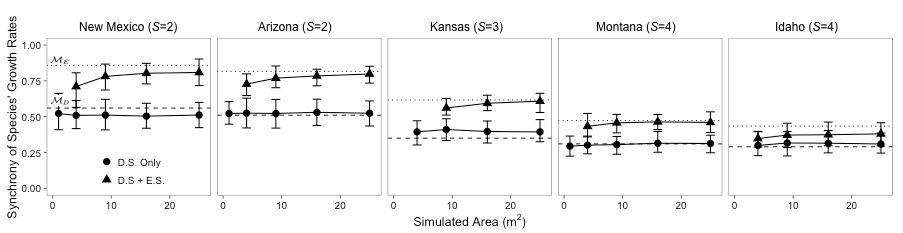
\includegraphics[width=6in]{./components/formatted_figures/formatted_figure2.png}
  \caption{Synchrony of species' growth rates for each study area from IBM simulations across different landscape sizes when only demographic stochastcity is present (``D.S. Only'') and when environmental stochasticity is also present removed (``D.S. + E.S.''). The horizontal lines show the analytical predictions $\mathcal{M}_D$ (dashed line) and $\mathcal{M}_E$ (dotted line). The strength of demographic stochasticity decreases as landscape size increases because population sizes also increase. Theoretically, ``D.S. Only'' simulations should remain constant across landscape size, whereas ``D.S. + E.S.'' simulations should shift from the $\mathcal{M}_D$ prediction to the $\mathcal{M}_E$ prediction as landscape size, and thus population size, increases, but only if demographic stochasticity it strong enough to counteract environmental forcing. Error bars represent the upper and lower 95\% quantiles from model simulations.}
\end{figure}

\pagebreak{}

\begin{figure}[!ht]
  \centering
      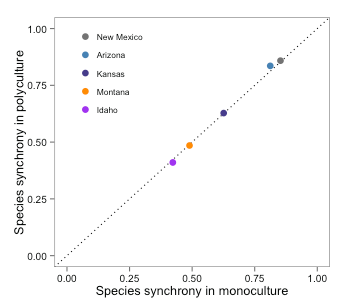
\includegraphics[width=4in]{./components/formatted_figures/formatted_figure3.png}
  \caption{Synchrony of species per capita growth rates simulated in large monocultures (IPM without species interactions) versus synchrony in large polycultures (IPM with species interactions). We used the same sequence of random year effects for both simulations (monoculture and polyculture) to mimic biodiversity-ecosystem functioning experiments. The dashed line is the line of equality. Simulation results in this figure are analogous to ``No Comp. + No D.S.'' (monocultures) and ``No D.S.'' (polycultures) in Fig. 1, but here we control the time series of random year effects.}
\end{figure}

\pagebreak{}



\end{document}
